\documentclass[a4paper]{extarticle}
\usepackage[left=2cm,top=2cm,right=2cm,bottom=2cm]{geometry}

\usepackage[utf8]{inputenc} % Eingabekodierung
\usepackage[T1]{fontenc}    % Besserer Umgang mit Sonderzeichen und Schriftarten
\usepackage[ngerman]{babel} % Bessere Unterstützung für deutsch
\usepackage{ulem}           % Textunterstreichungen

\usepackage{titlesec}       % Section-Stil: z.B. Farben

\usepackage{float}

\usepackage{tabularx}       % Tabellen mit mehr Optionen
\usepackage{listings}       % Darstellung von Programmcode mit Syntaxhervorhebung

\usepackage{tikz}           % Bildchen und Grafiken
\usepackage{tikz-qtree}
\usepackage{pgfplots}       % Graphen
\usepackage{graphicx}       % Bilder einfügen

\usepgfplotslibrary{colorbrewer,statistics}
\usetikzlibrary{arrows,arrows.meta,automata,positioning,patterns}
\pgfplotsset{compat=newest} % warum 

\usepackage{enumitem}       % Spezifizierung des Zählers bei Aufzählungen 
\usepackage{multirow}       % Tabellenunterteilungen
\usepackage{hyperref}       % Referenzen

\usepackage{algorithmicx}   % Grundgerüst, um Pseudocode-Strukturen zu definieren. 
\usepackage{algorithm}      % Floatumgebung

\usepackage{amsmath}        % Weitere Matheumgenungen und Möglichkeiten
\usepackage{amssymb}        % N Haufen Symbole
\usepackage{amsthm}         % Theoremumgebungen
\usepackage{gauss}          % Matrizen für einfache Pfeildarstellung von Spalten- und Zeilenumformungen

\usepackage[colorinlistoftodos,prependcaption,textsize=tiny]{todonotes} % todo
\usepackage{abstract}       % Zusammenfassungen



% Mathematik Definitionen

    \DeclareMathAlphabet{\bbold}{U}{bbold}{m}{n}

    \DeclareMathAlphabet{\dutchcal}{U}{dutchcal}{m}{n}
    \SetMathAlphabet{\dutchcal}{bold}{U}{dutchcal}{b}{n}
    \DeclareMathAlphabet{\dutchbcal}{U}{dutchcal}{b}{n}

    %  Kurzschreibweisen für Makros und Symbole
    \newcommand{\N}{\mathbb{N}}
    \newcommand{\R}{\mathbb{R}}
    \newcommand{\Q}{\mathbb{Q}}
    \newcommand{\Z}{\mathbb{Z}}
    \newcommand{\C}{\mathbb{C}}
    \newcommand{\bbF}{\mathbb{F}}
    \newcommand{\bbP}{\mathbb{P}}
    \newcommand{\bbV}{\mathbb{V}}
    \newcommand{\bbE}{\mathbb{E}}
    \newcommand{\calP}{\mathcal{P}}
    \newcommand{\calC}{\mathcal{C}}
    \newcommand{\calO}{\mathcal{O}}
    \newcommand{\calF}{\mathcal{F}}
    \newcommand{\calA}{\mathcal{A}}
    \newcommand{\calL}{\mathcal{L}}

    \newcommand{\calm}{\dutchcal{n}}
    \newcommand{\caln}{\dutchcal{m}}
    \newcommand{\call}{\dutchcal{l}}
    \newcommand{\cali}{\dutchcal{i}}
    \newcommand{\calj}{\dutchcal{j}}
    \newcommand{\calk}{\dutchcal{k}}

    \DeclareMathOperator{\bild}{bild}
    \DeclareMathOperator{\rang}{rang}
    \DeclareMathOperator{\grad}{grad}
    \DeclareMathOperator{\ggT}{ggT}
    \DeclareMathOperator{\arsinh}{arsinh}
    \DeclareMathOperator{\arcosh}{arcosh}
    \DeclareMathOperator{\artanh}{artanh}
    \DeclareMathOperator{\DSPACE}{DSPACE}
    \DeclareMathOperator{\NSPACE}{NSPACE}
    \DeclareMathOperator{\DTIME}{DTIME}
    \DeclareMathOperator{\NTIME}{NTIME}

    \newcommand{\partialto}{\rightharpoonup}
    \newcommand{\tr}{\mathsf{T}}

    \newcommand{\notiff}{\mathrel{{\ooalign{\hidewidth$\not\phantom{"}$\hidewidth\cr$\iff$}}}}
    \newcommand{\defiff}{\ :\Longleftrightarrow \ }
    \renewcommand{\land}{\hspace{1mm} \wedge \hspace{1mm}}
    \renewcommand{\lor}{\hspace{1mm} \vee \hspace{1mm}}

    \renewcommand{\le}{\leqslant}
    \renewcommand{\ge}{\geqslant}
    \renewcommand{\leq}{\leqslant}
    \renewcommand{\geq}{\geqslant}
    \newcommand{\isomorphic}{\cong}
    \newcommand{\congruent}{\equiv}

    %  Identische Abbildungen für Beschriftungen der Pfeile
    %  
    %  \rowops
    %  \add[<text oben>][<text unten>]01
    \renewcommand{\rowmultlabel}[1]{#1}
    \renewcommand{\colmultlabel}[1]{#1}
    \renewcommand{\rowswapfromlabel}[1]{#1}
    \renewcommand{\colswapfromlabel}[1]{#1}
    \renewcommand{\rowswaptolabel}[1]{#1}
    \renewcommand{\colswaptolabel}[1]{#1}
    \renewcommand{\rowaddfromlabel}[1]{#1}
    \renewcommand{\coladdfromlabel}[1]{#1}
    \renewcommand{\rowaddtolabel}[1]{#1}
    \renewcommand{\coladdtolabel}[1]{#1}

    %  \begin{gmatrix}{X} Für eckige Klammern
    \newmatrix{[}{]}{X}

    %  Umgebungen für Mathematische Aussagen. Angepasst an Subsection Nummerierung.
    \theoremstyle{definition}
    \newtheorem{subSatz}{Satz}[subsection]
    \newtheorem{subKorollar}{Korollar}[subSatz]
    \newtheorem{subLemma}[subSatz]{Lemma}
    \newtheorem{subDefinition}[subSatz]{Definition}
    \newtheorem{subBeispiel}[subSatz]{Beispiel}

    %  Umgebungen für Mathematische Aussagen. Angepasst an Section Nummerierung.
    \theoremstyle{definition}
    \newtheorem{secSatz}{Satz}[section]
    \newtheorem{secKorollar}{Korollar}[secSatz]
    \newtheorem{secLemma}[secSatz]{Lemma}
    \newtheorem{secDefinition}[secSatz]{Definition}
    \newtheorem{secBeispiel}[secSatz]{Beispiel}
    \newcommand{\theoremTitle}[1]{#1\vspace{0.1cm}}

    %  Kurzschreibweise Array 
    %
    %  \arr{c|c}{
    %      1 & -1\\  
    %      2 &  0\\ 
    %  }
    \newcommand{\arr}[2] {
        \begin{array}{#1} #2 \end{array}
    }

    %  Kurzschreibweise Matrix mit eckigen Klammern
    %
    %  \mat{
    %      1 & 1 & -1\\  
    %      2 & 3 &  0\\ 
    %  }
    \newcommand{\mat}[1] {
        \begin{bmatrix} #1 \end{bmatrix}
    }
    \newcommand{\smallmat}[1] {
        \left[\begin{smallmatrix} #1 \end{smallmatrix}\right]
    }
    \renewcommand{\vec}{\overset{\smash{\raisebox{-1.3pt}{\tiny{$\rightharpoonup$}}}}}

    %  LGS-Matrix mit Beschriftung
    %
    %  \gaussarr{cc}{
    %      1 & 1 & -1\\  
    %      2 & 3 &  0\\ 
    %  }{
    %      \\ -2 \cdot I\\ 
    %  }
    \newcommand{\gaussarr}[3] {
        \left[\arr{#1|c}{#2}\right]
        \arr{c}{#3}
    }

    %  Analog zu Stackrel aber besser für Text
    %
    %  \stackrelTiny{def}{=}
    \newcommand{\stackrelTiny}[2] {
        \stackrel{\text{\tiny{#1}}}{#2}
    }

% Mathematik Ende

% Text Kurzschreibweisen Definitionen

    \definecolor{light_blue}{rgb}{0.3, 0.4, 0.6}
    \definecolor{grey}{rgb}{0.3, 0.3, 0.3}
    \definecolor{light_grey}{rgb}{0.5, 0.5, 0.5}
    \definecolor{light_red}{rgb}{0.9, 0.3, 0.3}
    \definecolor{codegreen}{rgb}{0.1, 0.5, 0.1}

    \newcommand{\blueit}[1]{\textit{\textcolor{light_blue}{#1}}}
    \newcommand{\bluebf}[1]{\textbf{\textcolor{light_blue}{#1}}}
    \newcommand{\blueitbf}[1]{\textit{\textbf{\textcolor{light_blue}{#1}}}}
    \renewcommand{\t}[1]{\text{#1}}

    \newcommand{\tab}{\hspace*{0.25cm}}
    \newcommand{\bigtab}{\hspace*{0.50cm}}

% Text Kurzschreibweisen Ende

% Algorithmen Definitionen

    %  \begin{algorithm}
    %      \caption{Algorithm}
    %      \begin{algorithmic}[1]
    %          \Procedure{run}{a,b}
    %              \If{$a = b$} 
    %                  \State a := 2
    %              \EndIf
    %              \Return a
    %          \EndProcedure
    %      \end{algorithmic}
    %  \end{algorithm}    
    \algblockdefx[IF]{IF}{ENDIF}[1]{\textbf{IF} #1 \textbf{DO}}{\textbf{END}}
    \algcblockdefx[ELSEIF]{IF}{ELSEIF}{ENDIF}[1]{\textbf{ELSE IF} #1 \textbf{DO}}{\textbf{END}}
    \algcblockdefx[ELSE]{ELSEIF}{ELSE}{ENDIF}{\textbf{ELSE}}{\textbf{END}}
    \algcblockdefx[ELSE]{IF}{ELSE}{ENDIF}{\textbf{ELSE}}{\textbf{END}}

    \algblockdefx[WHILE]{WHILE}{ENDWHILE}[1]{\textbf{WHILE} #1 \textbf{DO}}{\textbf{END}}
    \algblockdefx[FOR]{FOR}{ENDFOR}[2]{\textbf{FOR} #1 \textbf{TO} #2 \textbf{DO}}{\textbf{END}}
    \algblockdefx[LOOP]{LOOP}{ENDLOOP}[1]{\textbf{LOOP} #1 \textbf{DO}}{\textbf{END}}
    \algblockdefx[FOREACH]{FOREACH}{ENDFOR}[1]{\textbf{FOR EACH} #1 \textbf{DO}}{\textbf{END}}

    \algblockdefx[PROCEDURE]{PROCEDURE}{ENDPROCEDURE}[2]{\textbf{PROCEDURE} \textsc{#1}(#2)}{\textbf{END PROCEDURE}}

    \newcommand{\RETURN}{\State \textbf{RETURN }}

    \algblockdefx[If]{If}{EndIf}[1]{\textbf{if} #1 \textbf{do}}{\textbf{end}}
    \algcblockdefx[ElseIf]{If}{ElseIf}{EndIf}[1]{\textbf{else if} #1 \textbf{do}}{\textbf{end}}
    \algcblockdefx[Else]{ElseIf}{Else}{EndIf}{\textbf{else}}{\textbf{end}}
    \algcblockdefx[Else]{If}{Else}{EndIf}{\textbf{else}}{\textbf{end}}

    \algblockdefx[While]{While}{EndWhile}[1]{\textbf{while} #1 \textbf{do}}{\textbf{end}}
    \algblockdefx[For]{For}{EndFor}[2]{\textbf{for} #1 \textbf{to} #2 \textbf{do}}{\textbf{end}}
    \algblockdefx[ForEach]{ForEach}{EndFor}[1]{\textbf{for each} #1 \textbf{do}}{\textbf{end}}
    \algblockdefx[Loop]{Loop}{EndLoop}[1]{\textbf{loop} #1 \textbf{do}}{\textbf{end}}

    \algblockdefx[Procedure]{Procedure}{EndProcedure}[2]{\textbf{procedure} \textsc{#1}(#2)}{\textbf{end procedure}}
    \algblockdefx[Function]{Function}{EndFunction}[2]{\textbf{fn} {#1}(#2) := $\{$}{\textbf{$\}$}}

    \newcommand{\Return}{\State \textbf{return }}

% Algorithmen Ende

% Titel und Seitenformat Definitionen

    \newcommand{\onpageTitleSubtitle}[2]{
        \begin{center}
            \huge{\textbf{#1}}

            \normalsize{#2}
        \end{center}
    }
    \newcommand{\onpageTitle}[1]{
        \begin{center}
            \huge{\textbf{#1}}
        \end{center}
    }
    \newcommand{\sectionColor}[1] {
        \titleformat{\section}
            {\color{#1}\normalfont\Large\bfseries}
            {\color{#1}\thesection}{1em}{}
        \titleformat{\subsection}
            {\color{#1}\normalfont\large\bfseries}
            {\color{#1}\thesubsection}{1em}{}
        \titleformat{\subsubsection}
            {\color{#1}\normalfont\normalsize\bfseries}
            {\color{#1}\thesubsubsection}{1em}{}
    }
    

% Ende Titel und Seitenformat

% Praktische Umgebungen Definitionen

    \newcounter{secnotecounter}[section]

    \newenvironment{secNote}[1] {
        \refstepcounter{secnotecounter}
        \begin{center}
        \begin{tabular}{|c|}
        \hline
        \begin{minipage}[b][][t]{0.95\columnwidth}
        \vspace*{0.15cm} \textbf{\thesection.\thesecnotecounter \ #1}
    } {
        \end{minipage}
        \\\hline
        \end{tabular}
        \end{center}
    }

    \newcounter{notecounter}[subsection]

    \newenvironment{subNote}[1] {
        \refstepcounter{notecounter}
        \begin{center}
        \begin{tabular}{|c|}
        \hline
        \begin{minipage}[b][][t]{0.95\columnwidth}
        \vspace*{0.15cm} \textbf{\thesection.\thesubsection.\thenotecounter \ #1}
    } {
        \end{minipage}
        \\\hline
        \end{tabular}
        \end{center}
    }

    \newenvironment{textbox} {
        \begin{center}
        \begin{tabular}{|c|}
        \hline
        \begin{minipage}[b][][t]{0.95\columnwidth}
        \vspace*{0.15cm}
    } {
        \end{minipage}
        \\\hline
        \end{tabular}
        \end{center}
    }

    \tikzset{ALL_STATE/.style = {rectangle, minimum size = 0.8cm, draw = black!100}}
    \tikzset{EXS_STATE/.style = {circle, state}}
    \newenvironment{automaton}[1] {
        \begin{tikzpicture}[node distance = #1, ->, > = stealth]
    } {
        \end{tikzpicture}
    }

% Ende Praktische Umgebungen

% Listings: Hübsche Stile

    \definecolor{clr-background}{RGB}{255,255,255}
    \definecolor{clr-text}{RGB}{0,0,0}
    \definecolor{clr-string}{RGB}{161, 34, 8}
    \definecolor{clr-namespace}{RGB}{0,0,0}
    \definecolor{clr-preprocessor}{RGB}{100, 100, 100}
    \definecolor{clr-keyword}{RGB}{0,0,255}
    \definecolor{clr-type}{RGB}{30, 110, 240}
    \definecolor{clr-variable}{RGB}{0,0,0}
    \definecolor{clr-constant}{RGB}{111,0,138}
    \definecolor{clr-comment}{RGB}{160, 110, 90}
    \definecolor{clr-identifier}{RGB}{143, 139, 113}

    \lstset{literate=
        {Ö}{{\"O}}1
        {Ä}{{\"A}}1
        {Ü}{{\"U}}1
        {ß}{{\ss}}1
        {ü}{{\"u}}1
        {ä}{{\"a}}1
        {ö}{{\"o}}1
        {~}{{\textasciitilde}}1
    }
    \lstset{emph={Thing}}

    % C++ Stiele: TODO: Aufräumen

    \lstdefinestyle{cpp_fabio}{
        language=C++,
        frame=tb,
        backgroundcolor=\color{clr-background}\footnotesize\ttfamily,
        basicstyle=\color{clr-text}\footnotesize\ttfamily,
        stringstyle=\color{clr-string}\footnotesize\ttfamily,
        identifierstyle=\color{clr-variable}\footnotesize\ttfamily,
        commentstyle=\color{clr-comment}\footnotesize\ttfamily,
        directivestyle=\color{clr-preprocessor}\footnotesize\ttfamily,
        keywordstyle=\color{clr-type}\footnotesize\ttfamily,
        keywordstyle={[2]\color{clr-constant}},
        showstringspaces=false,
        numbers=left,
        % identifierstyle=\color{clr-identifier},
        morekeywords={Thing, string},
        tabsize=4
    }

    \lstdefinestyle{cpp_fabio_inline}{
        language=C++,
        frame=tb,
        backgroundcolor=\color{clr-background}\ttfamily,
        basicstyle=\color{clr-text}\ttfamily,
        stringstyle=\color{clr-string}\ttfamily,
        identifierstyle=\color{clr-variable}\ttfamily, 
        commentstyle=\color{clr-comment}\ttfamily,
        directivestyle=\color{clr-preprocessor}\ttfamily,
        keywordstyle=\color{clr-type}\ttfamily,
        keywordstyle={[2]\color{clr-constant}},
        % dentifierstyle=\color{clr-identifier},
        showstringspaces=false,
        morekeywords={Thing, string},
        tabsize=4
    }

    % In-Zeilen-Kode
    \newcommand{\code}[1] {\lstinline[style = cpp_fabio_inline]{#1}}

% Ende Listings

\setlength{\parindent}{0cm} % Einrückung bei Textblockanfang aus
\renewcommand{\arraystretch}{1.3}
\usepackage{abstract}

\begin{document}
    \begin{center}
        \huge
        \textbf{Forschungsprojekt: Wärmepumpendemonstrator}
            
        \vspace{0.4cm}
        \large
        Demonstratorapp zur Präsentierung der Ergebnisse eines Konvolutionsnetzwerks für Wärmepumpen
            
        \vspace{0.6cm}
        \normalsize
        \begin{tabular}{llll}
            Ursula Krause & (st$X$), & Laurin Röseler & (st177288),\\
            Christof Schuster & (st$X$), & Fabio Tucciarone & (st177167)
        \end{tabular}

        \vspace{0.3cm}
        st$X$@stud.uni-stuttgart.de
        
        \vspace{0.8cm}
    \end{center}

    \begin{abstract}
        Neque porro quisquam est qui dolorem ipsum quia dolor sit amet, consectetur, adipisci velit...
        Neque porro quisquam est qui dolorem ipsum quia dolor sit amet, consectetur, adipisci velit...
        Neque porro quisquam est qui dolorem ipsum quia dolor sit amet, consectetur, adipisci velit...
    \end{abstract}

    \section{Einführung}

    


    \section{Projektarchitektur}

    Zu Begin möchten wir einen Überblick über die Projektarchitektur und die dazugehörigen Entwurfsentscheidungen geben.
    

    \begin{itemize}
        \item Diagramm: Zusammenspiel der Komponenten (grob)
        \begin{figure}[H]
            \centering
            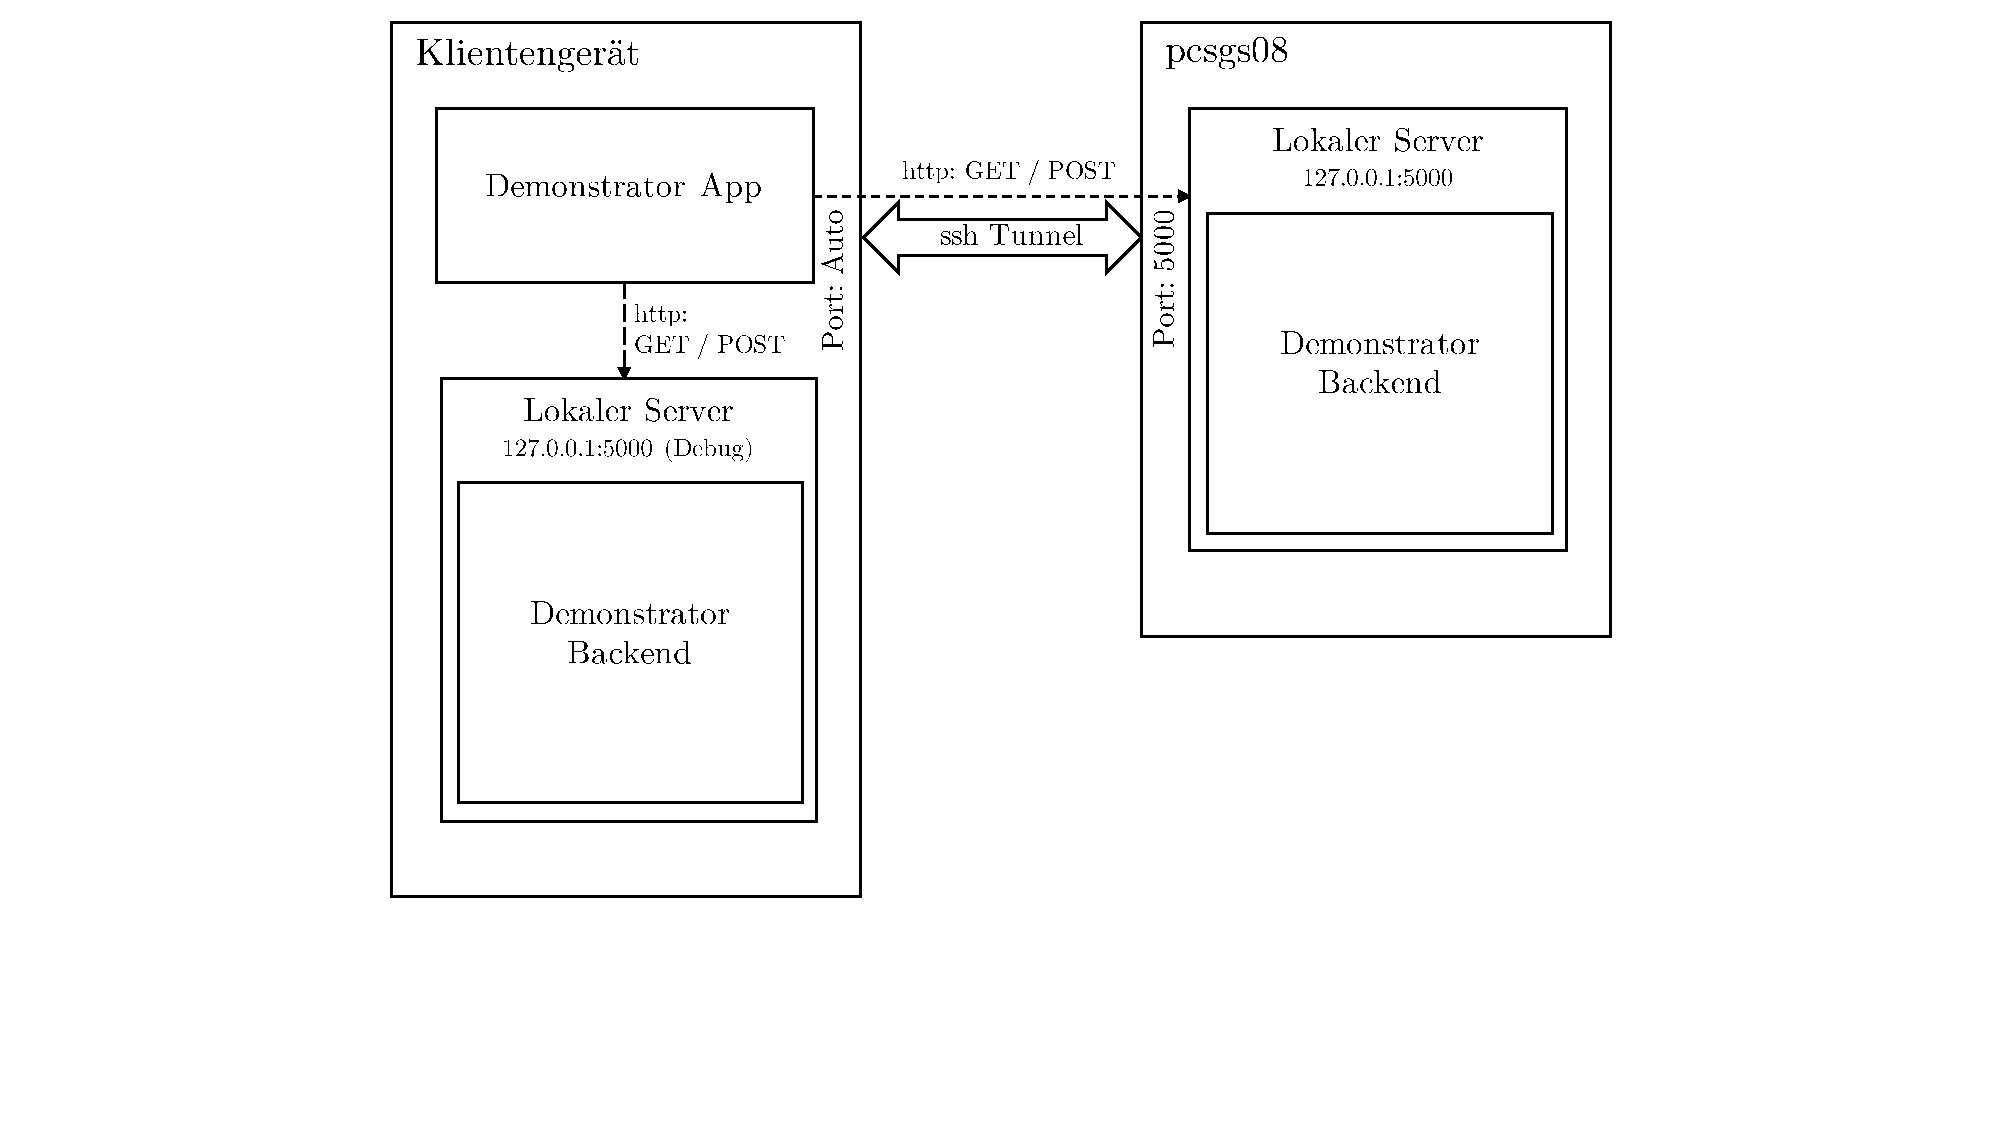
\includegraphics[trim={5cm 3.5cm 5cm 0}, clip, width=0.8\linewidth]{bilder/architektur_projekt.pdf}
            \caption{Grobe Projektarchitektur} \label{fig:architektur-projekt}
        \end{figure}
        \item Backend
        \begin{figure}[H]
            \centering
            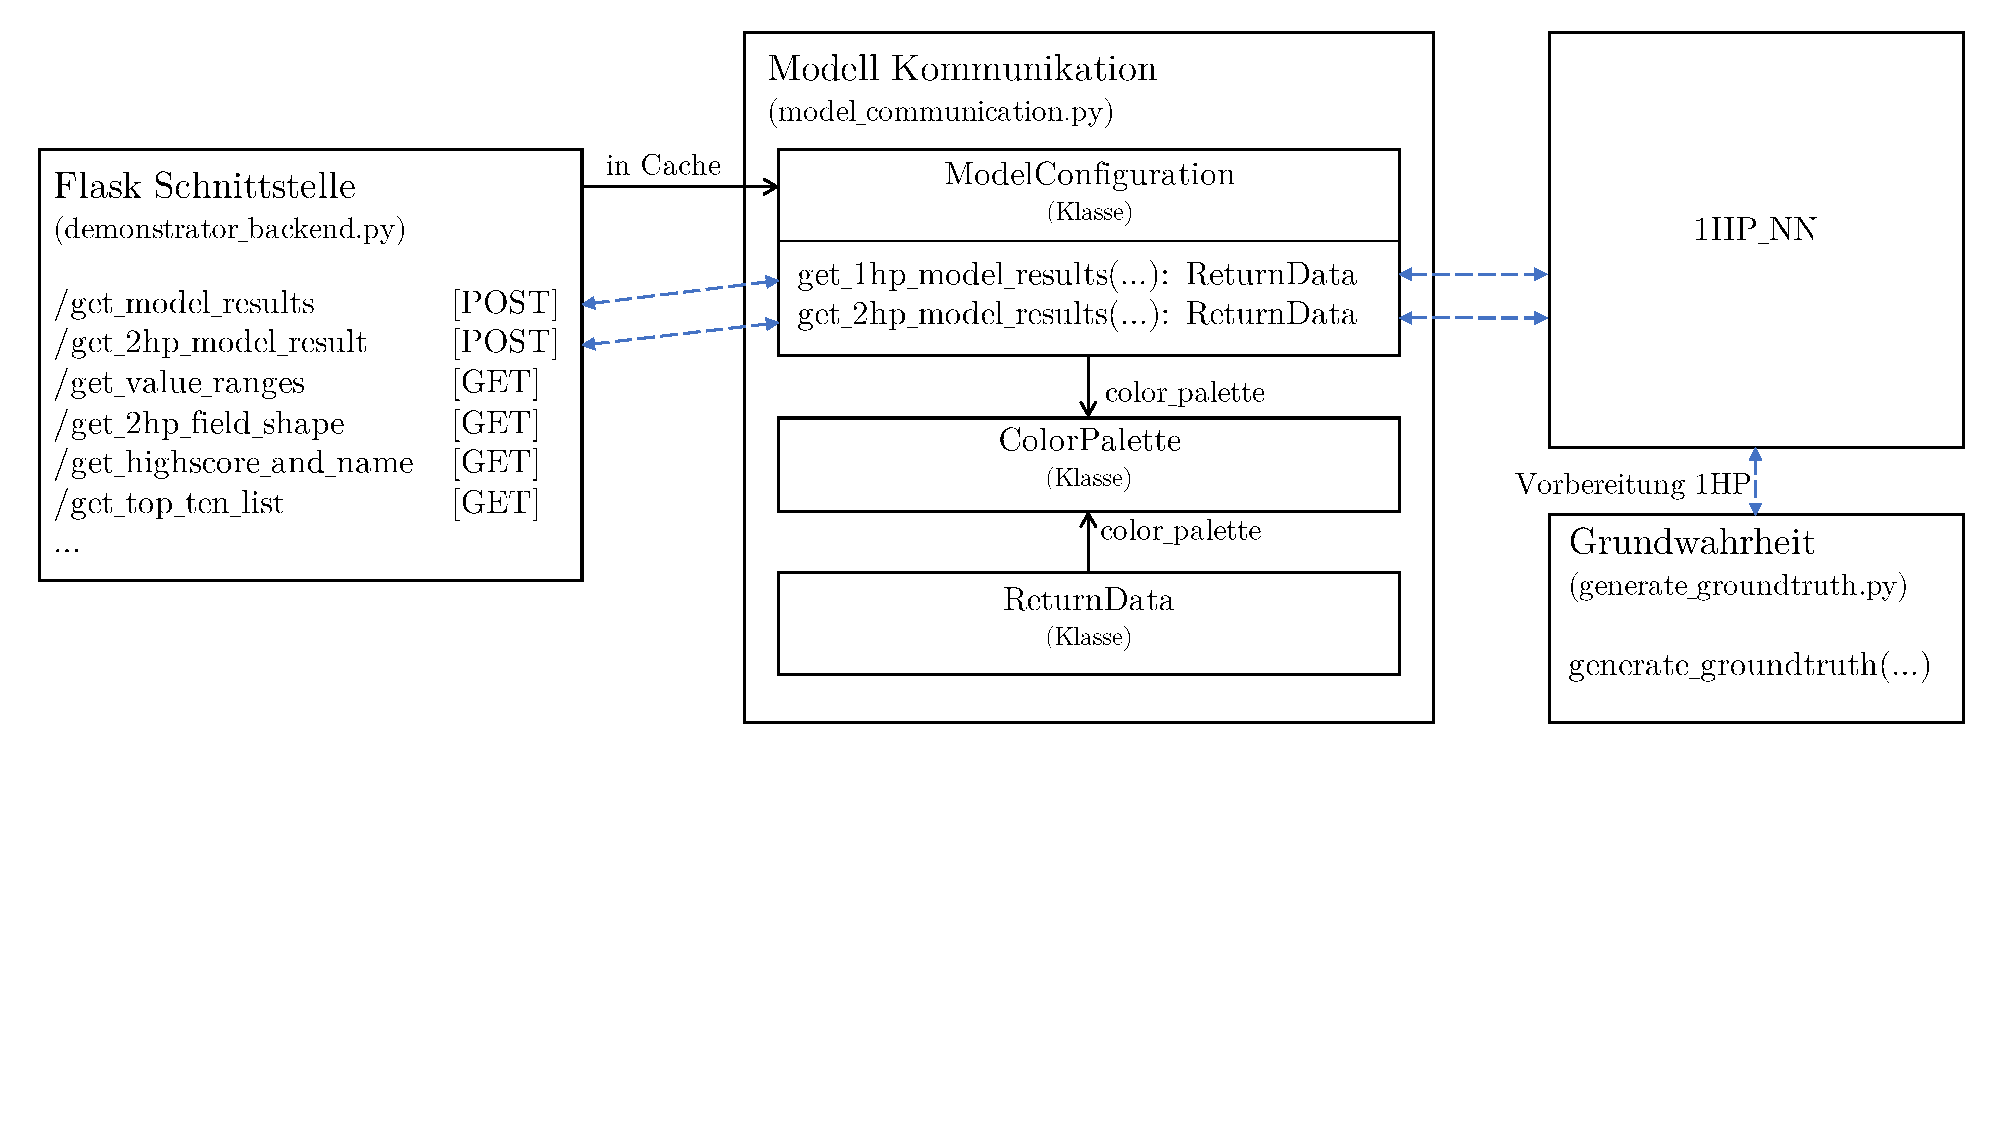
\includegraphics[trim={0cm 6cm 0cm 0}, clip, width=\linewidth]{bilder/architektur_backend.pdf}
            \caption{Grobe Projektarchitektur} \label{fig:architektur-backend}
        \end{figure}
        \item Frontend?
    \end{itemize}

    \section{Backend}
    \subsection{Stufe 1 (1HP NN)}
    \begin{itemize}
        \item Hauptaufgabe: Generierung einer Grundwahrheit für eine Wärmepumpe
        \begin{itemize}
            \item Algorithmus: Nächster Punkt
            \item Algorithmus: Scipy Versuche (Vergleiche: Laufzeit, Fehler)
            \item Algorithmus: Unser Algorithmus (Vergleiche ...)
        \end{itemize}
        \item Kommunikation mit dem Modell
        \begin{itemize}
            \item Pipeline / Ablauf einer Anfrage
            \item Optimierungen / Engpässe
        \end{itemize}
    \end{itemize}
    \subsubsection{Triangulation}
    % nächster Punkt bei Interpolanten, dabei gesucht: minimale Punktabstandssumme Wir wollen ein Dreieck aus drei Datenpunkten, $c, c_1$ und $c_2$ um einen Punkt $p$ legen.
    $Vor"uberlegung:$ Um die Farbe eines Pixels in einer zweidimensionalen Ebene zufällig verteilter
    Datenpunkte anzunähern, empfiehlt es sich über ein Dreieck aus Datenpunkten, das den Pixel 
    einschließt zu interpolieren. Dabei, um möglichst viel von den Informationen der Datenpunkte 
    zu nutzen, sollten die drei Datenpunkte einen möglichst geringen Abstand zum Pixelpunkt $p$ 
    besitzen. Die drei Datenpunkte, die das Dreieck bilden sollen, nennen wir $c, c_1$ und $c_2$.
    Bevor wir einen Algorithmus \ref{tri_k} konstruieren, der diese Eigenschaft erfüllt erst noch 
    wichtige Hilfssätze:

    \subsubsection{Hilfssatz 1: Minimales-Abstands-Dreieck beinhaltet nächsten Punkt} \label{tri_hs1}
    Damit ein solches Dreieck eine minimale Punktabstandssumme besitzt,
    ist es notwendig, dass der, zu $p$ nächste, Datenpunkt Teil dieses Dreiecks ist. Diesen Punkt 
    nennen wir $c$.

    \begin{figure*}[!ht]
        \centering	
        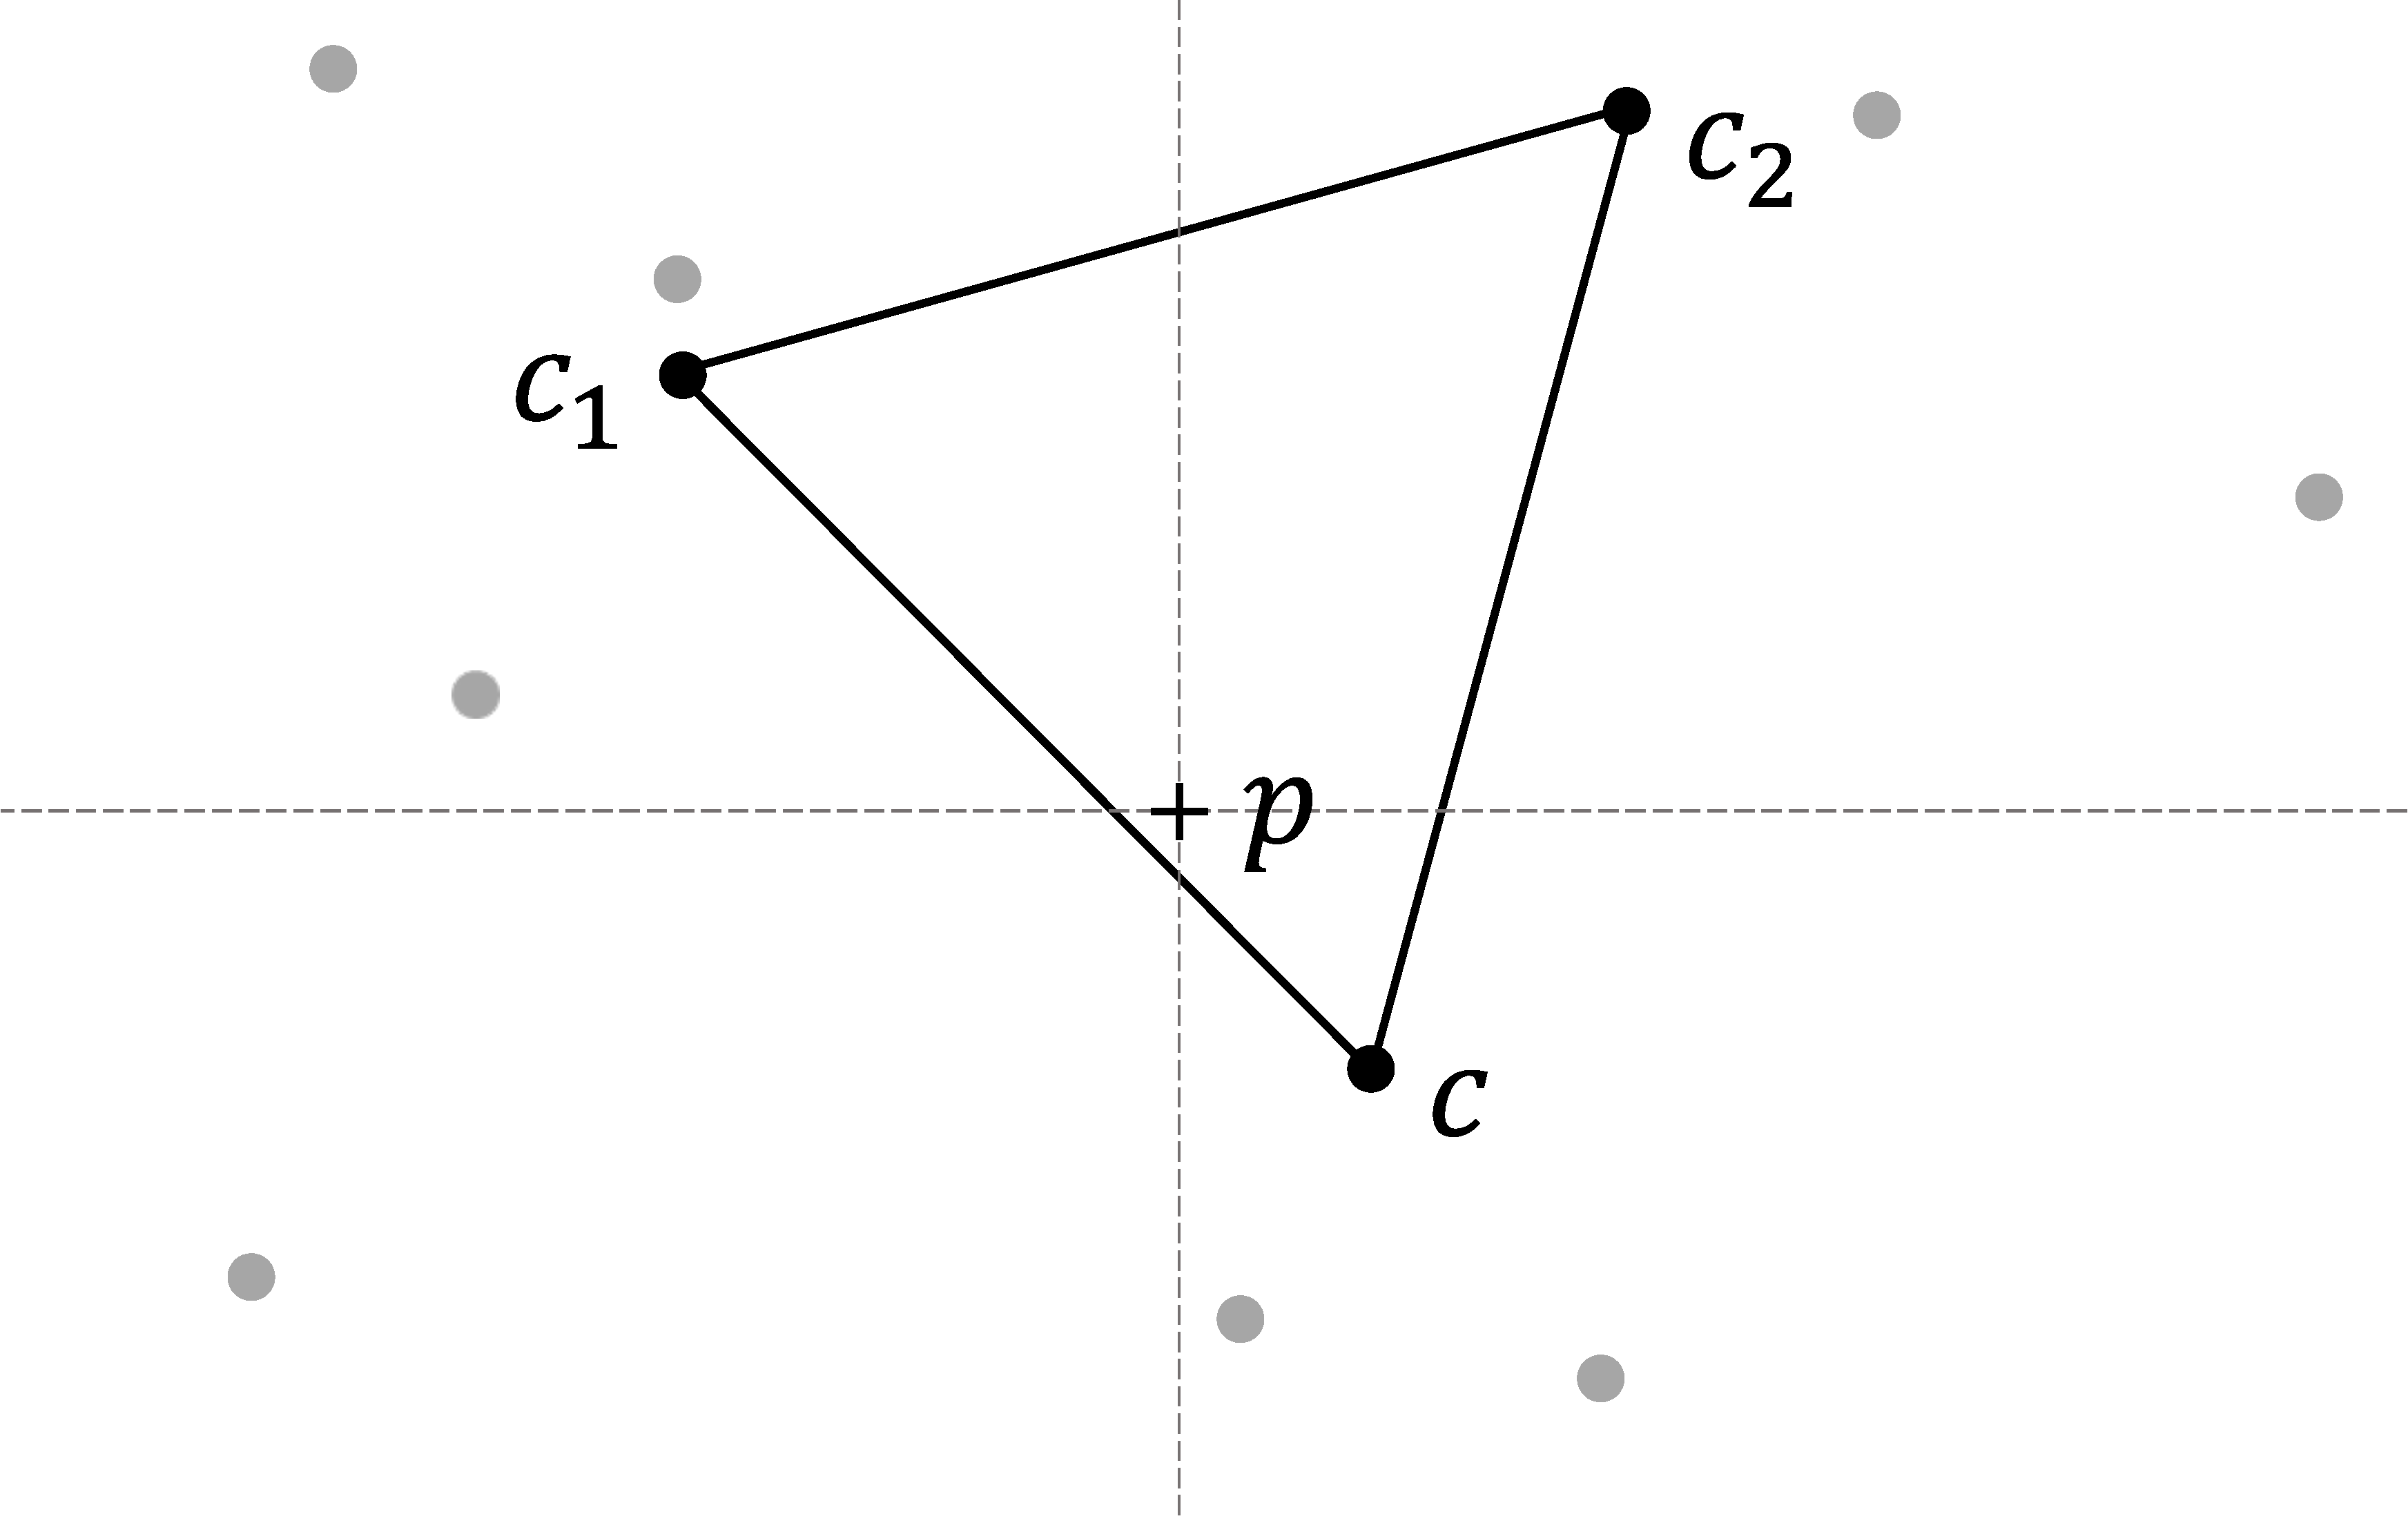
\includegraphics[scale=0.10]{bilder/tri_1.pdf}
        \caption{Ziel Triangulation}
        \label{fig:triangulation_1}
    \end{figure*}

    $Beweis:$
    Angenommen, $c$ wäre nicht Teil des $p$-umschließenden Dreiecks mit minimaler Punktabstandssumme.
    Dieses Dreieck bestehe aus den Eckpunkten $a_1$, $a_2$ und $a_3$ mit Abstandssumme:

    \begin{eqnarray*}
        S_{\text{AP}} &=& \mid p - a_1 \mid + \mid p - a_2 \mid + \mid p - a_3 \mid \\
    \end{eqnarray*}
    
    Von den drei Punkten sei $a_1$ der nächste Punkt zu $p$. Dieser spannt, mit $p$ als Mittelpunkt, 
    einen Kreis auf. Innerhalb davon muss $c$ liegen.
    Es gibt nun einen Punkt $\in \{ a_1, a_2, a_3 \}$, der sich durch $c$ ersetzen lässt und
    mit den anderen beiden Punkten ein Dreieck aufspannt, das immer noch $p$ umschließt 
    (siehe \ref{fig:triangulation_2}).

    \begin{figure*}[!ht]
        \centering	
        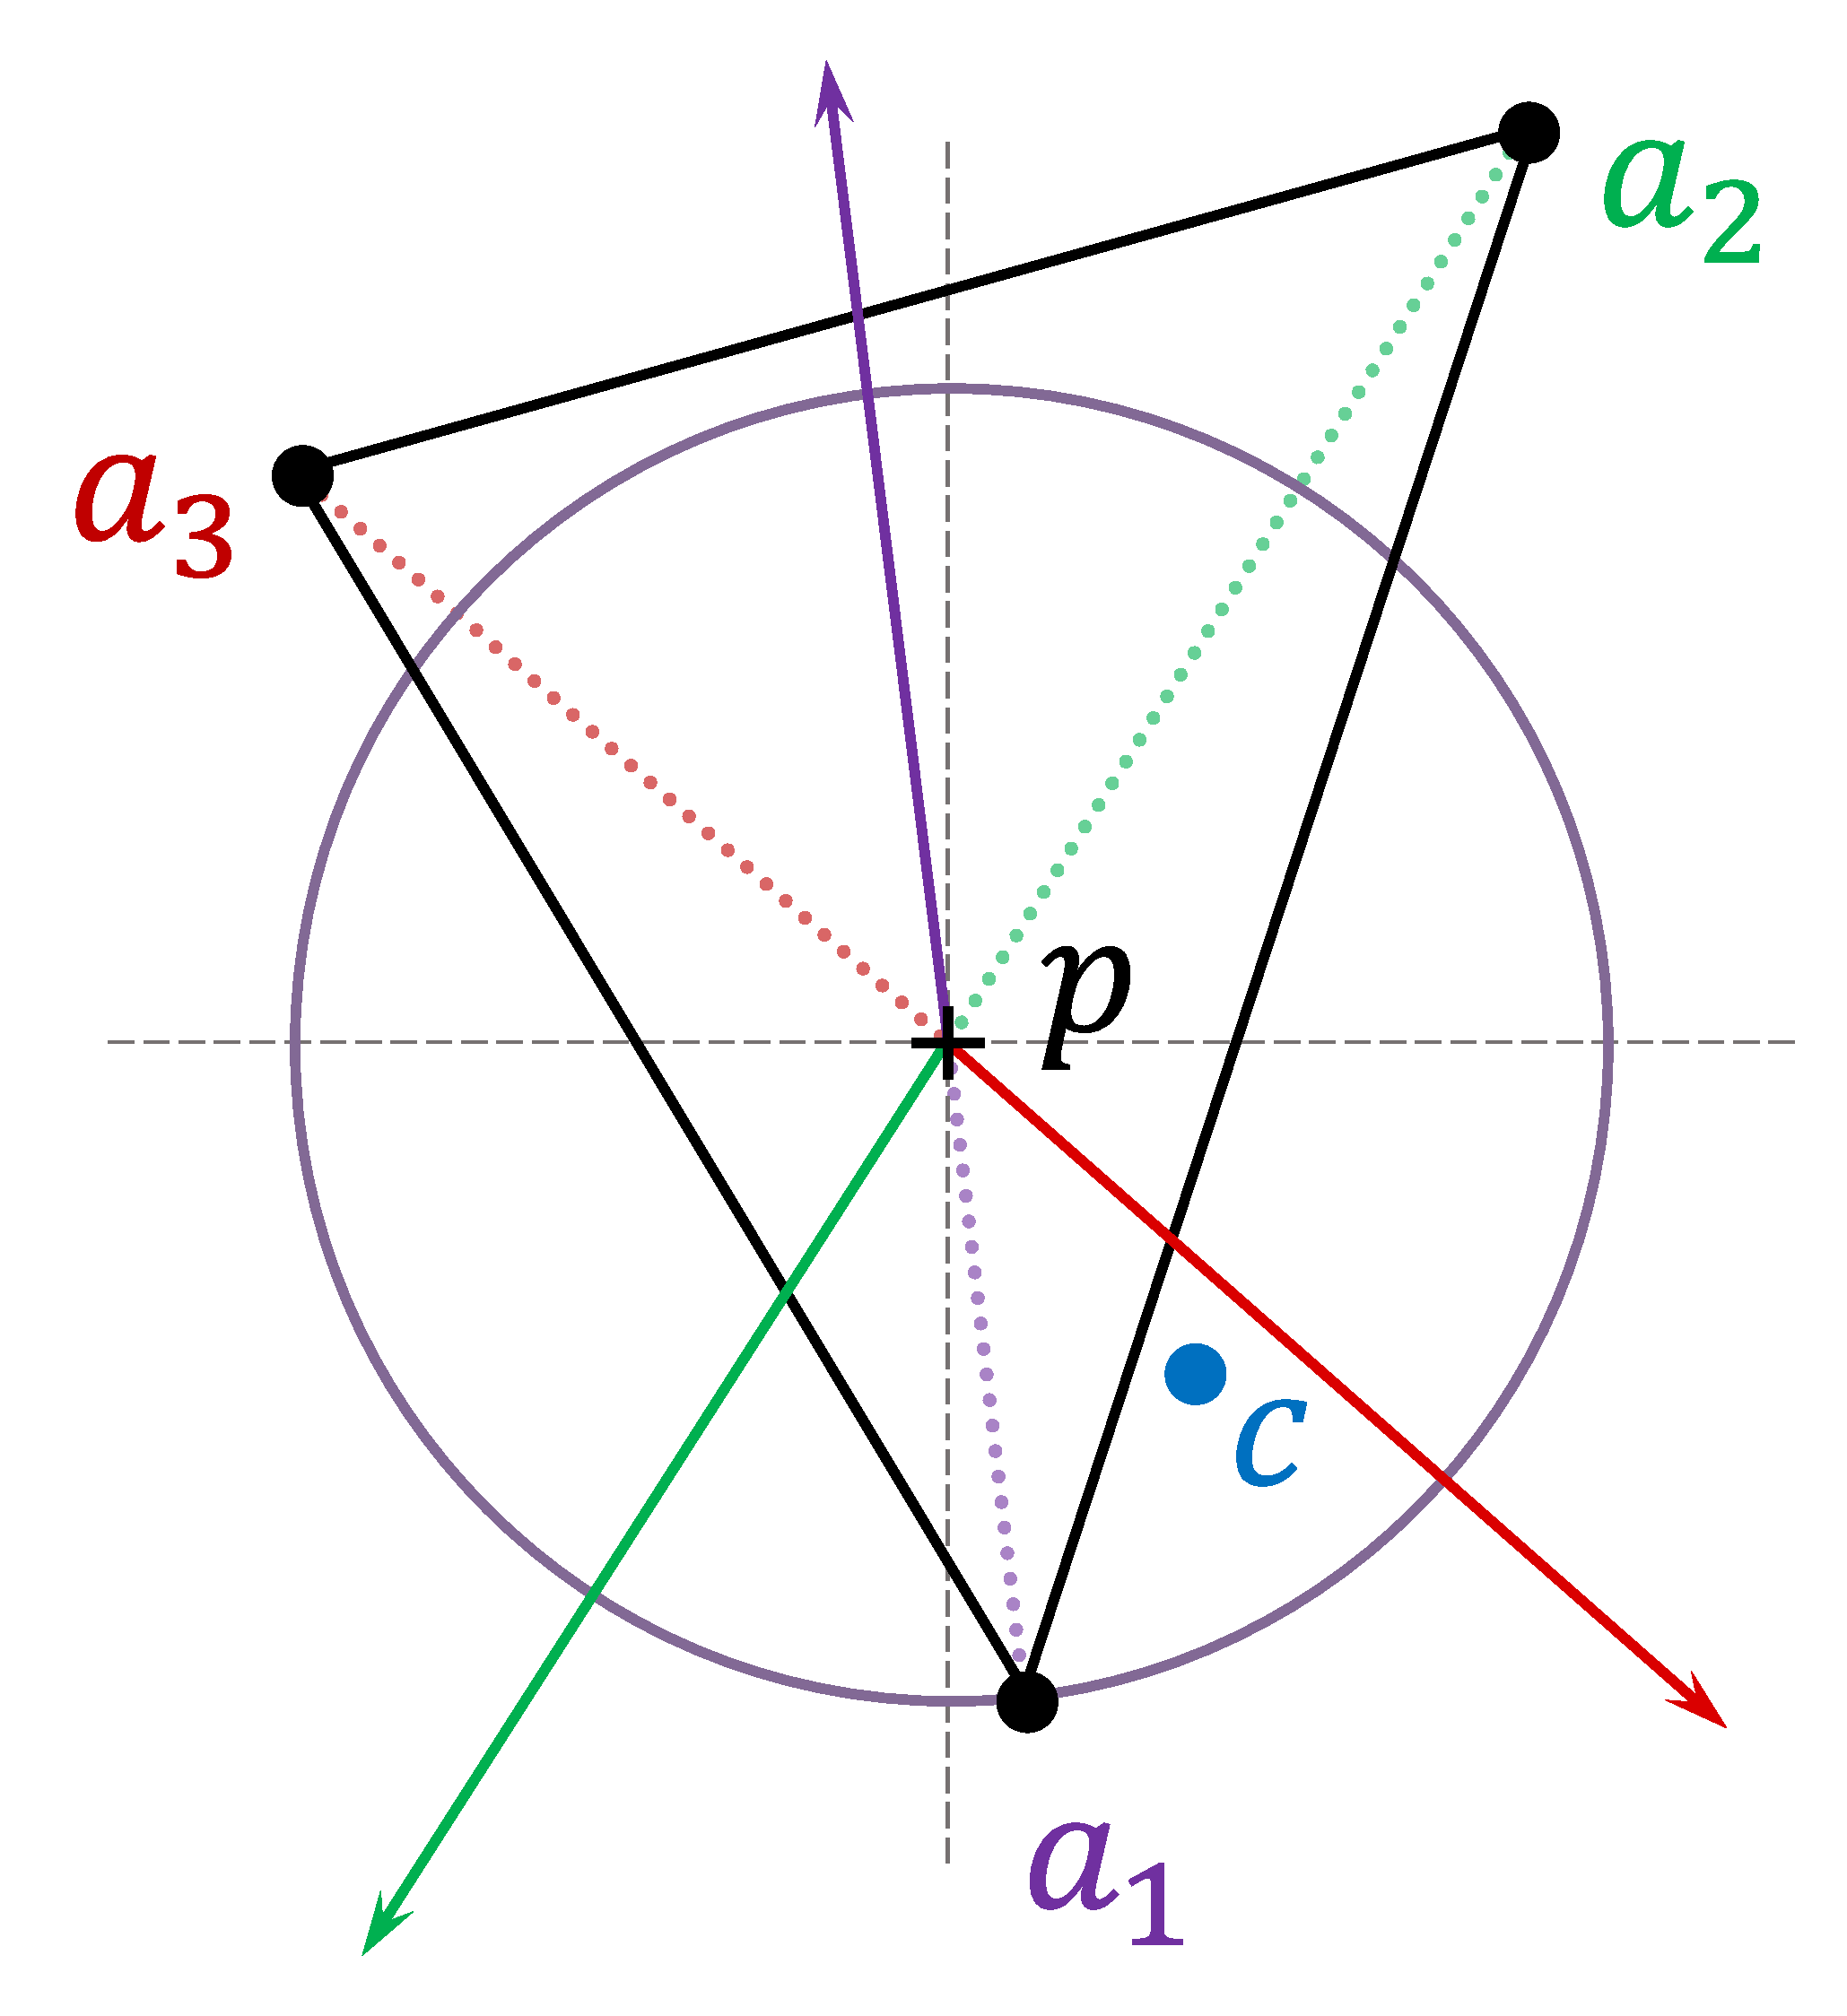
\includegraphics[scale=0.15]{bilder/tri_2.pdf}
        \caption{Dreiteilung mit Hilfslinien}
        \label{fig:triangulation_2}
    \end{figure*}

    Diesen, zu ersetzenden Punkt, kann man finden, indem man zuerst von jedem Punkt 
    $\in \{ a_1, a_2, a_3 \}$ eine Linie durch $p$ zieht (in Abb. \ref{fig:triangulation_2} lila, 
    grün, rot). Diese Linien, von $p$ ausgehend (nur noch die durchgezogenen Linien), teilen die 
    Ebene in drei Teile auf, wobei in jedem genau ein Punkt $\in \{ a_1, a_2, a_3 \}$ liegt.
    Wäre mehr als ein Punkt in einem Teil, so umschlössen die drei Punkte nicht mehr $p$ 
    (siehe \ref{tri_hs2}).

    \begin{figure*}[!ht]
        \centering	
        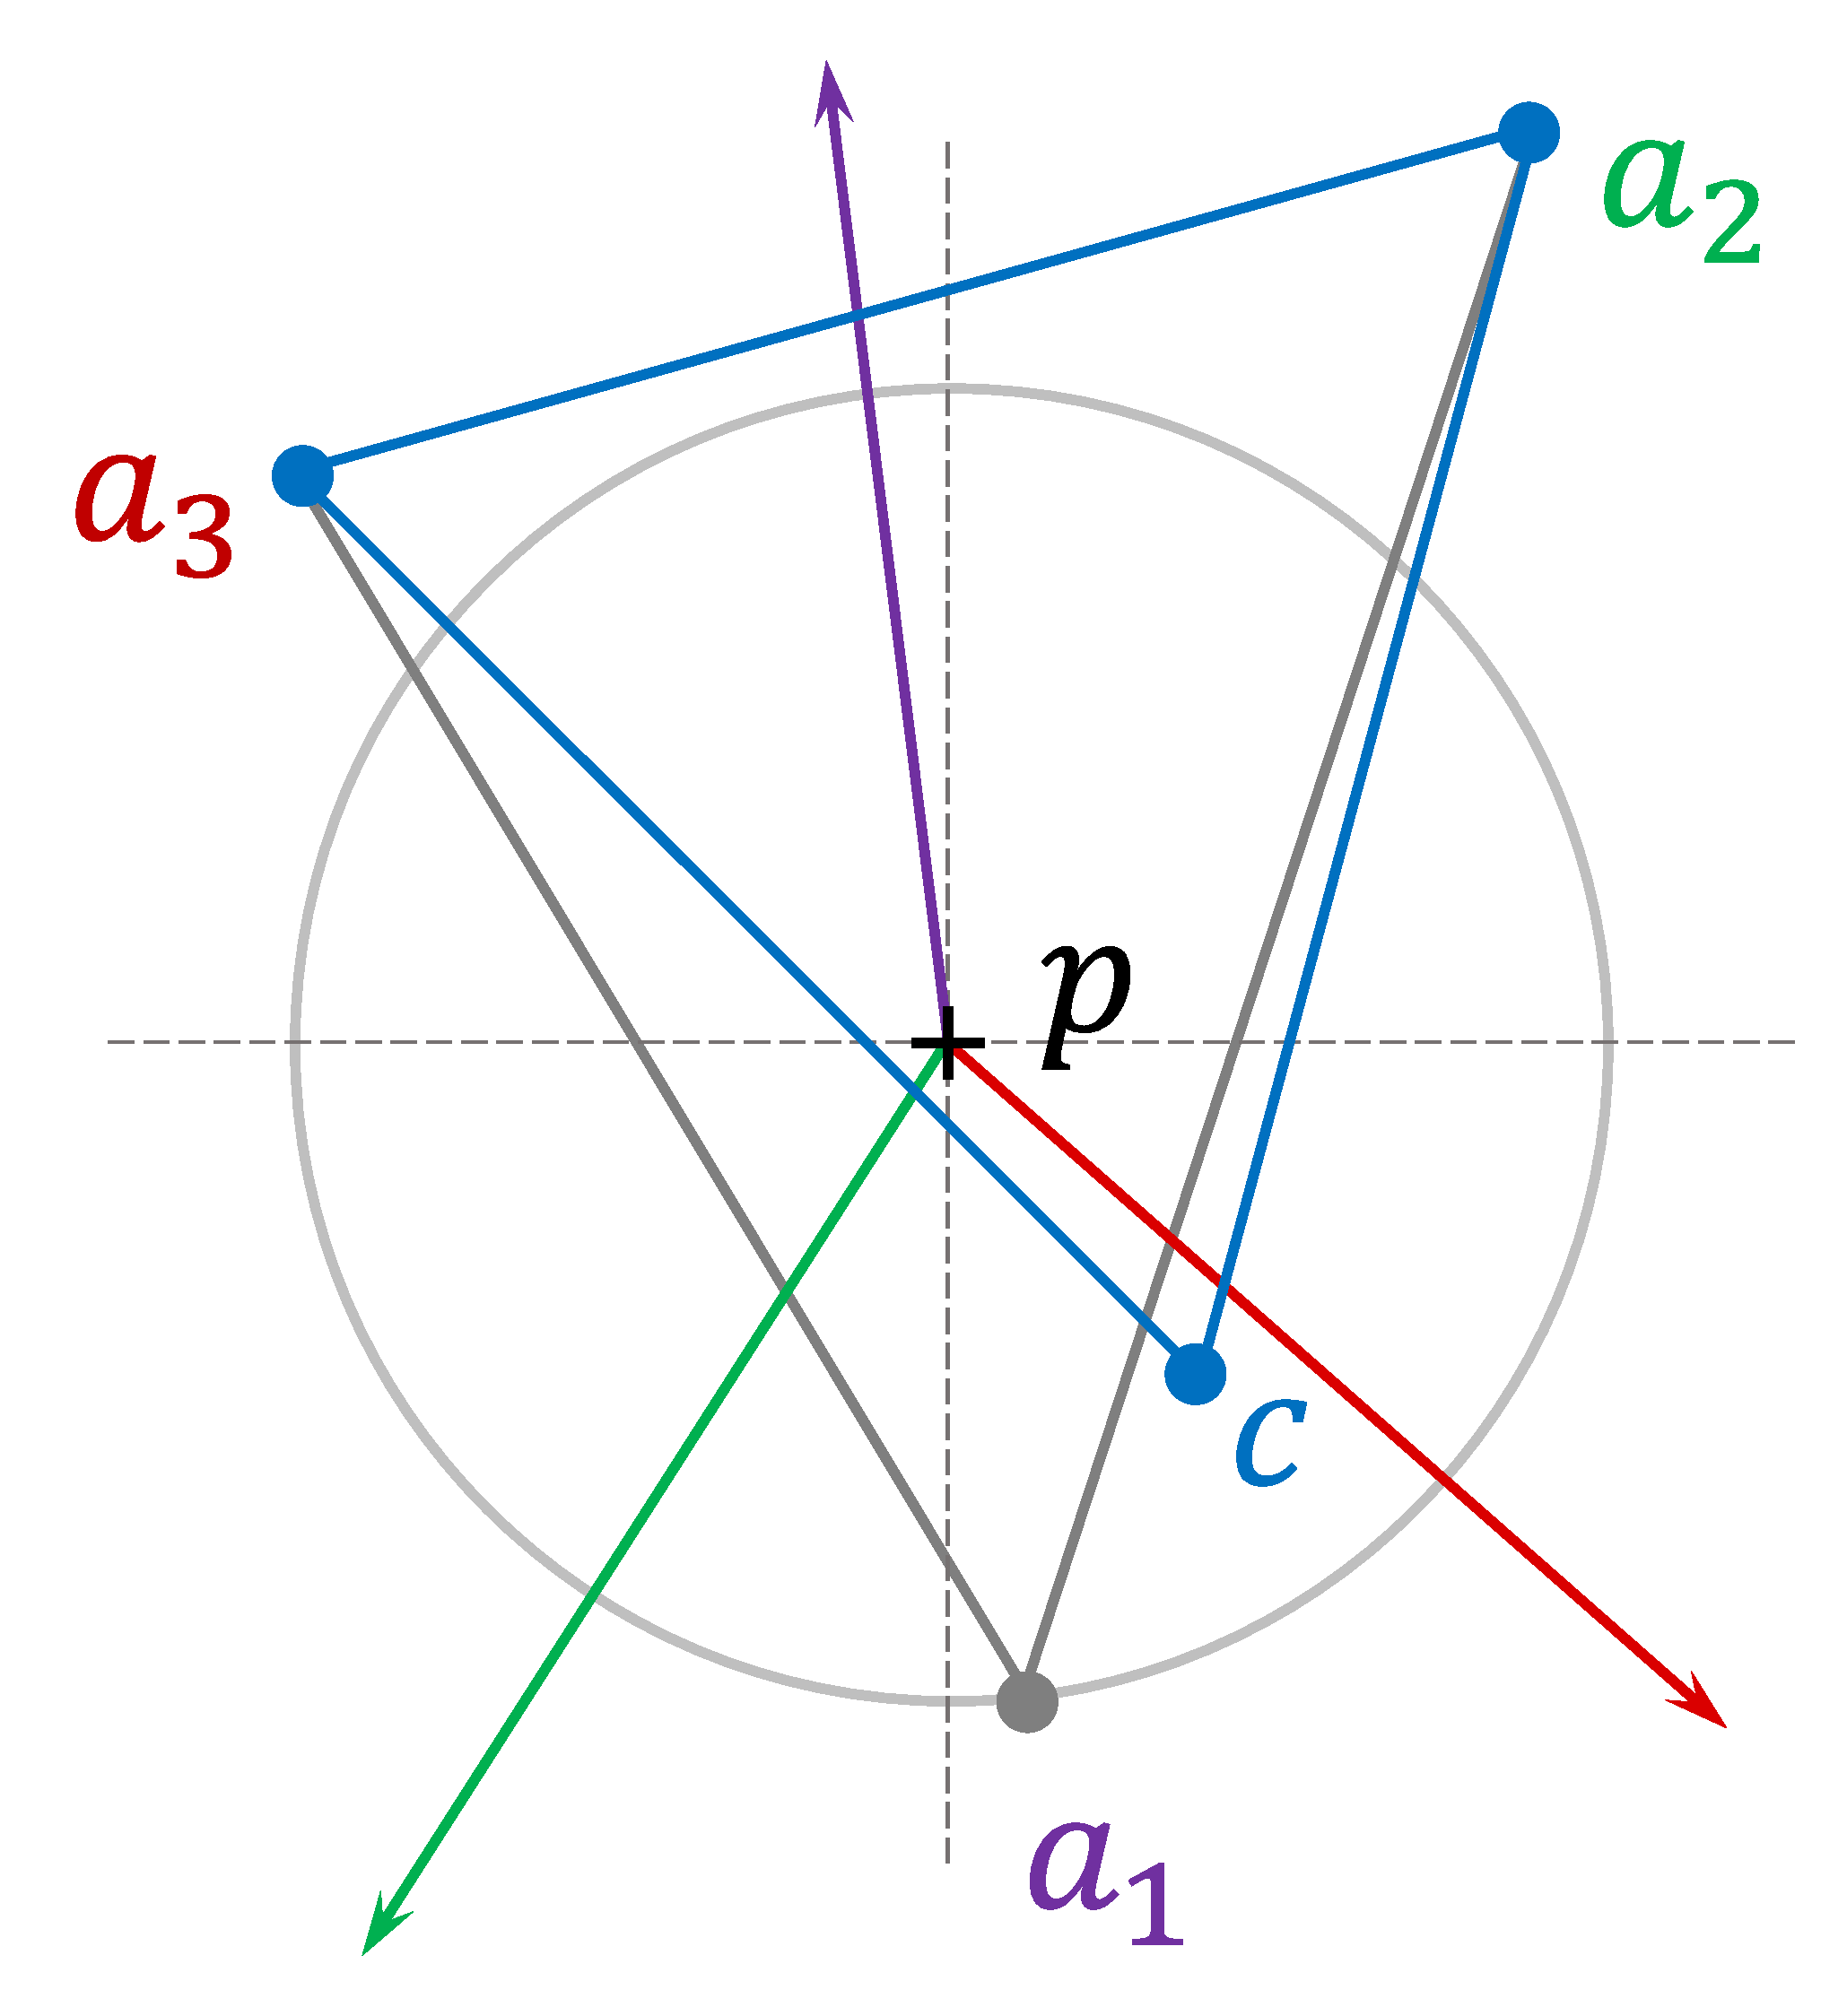
\includegraphics[scale=0.15]{bilder/tri_3.pdf}
        \caption{kleineres Dreieck}
        \label{fig:triangulation_3}
    \end{figure*}

    Sei $a_1$ der Punkt, der im selben Teil wie $c$ liegt. Dieser lässt sich durch $c$ ersetzen, 
    da jeder Punkt innerhalb dieses Teils, ein $p$ umschließendes Dreieck mit $a_2$ und $a_3$ 
    aufstellen würde. Das liegt daran, dass die Mindestgröße der 
    Winkel an jeweils $a_2$ und $a_3$ ausreicht, um $p$ zu umschließen (siehe \ref{tri_hs2}).
    Die Mindestgröße beider Winkel wird schließlich von dem Teil bestimmt, der $a_1$ beinhaltet.
    Das neue Dreieck ($c$,$a_2$,$a_3$) hat somit die Punktabstandssumme:

    \begin{eqnarray*}
        S^*_{\text{AP}} &=& \mid p - c \mid + \mid p - a_2 \mid + \mid p - a_3 \mid \\
    \end{eqnarray*}

    O.B.d.A: $S^*_{\text{AP}}$ ist kleiner als $S_{\text{AP}}$, da der Abstand von $c$ zu $p$
    kleiner ist als der von $a_1$ zu $p$. Das ist ein Widerspruch zur Annahme, dass ($a_1, a_2, a_3$) 
    das Dreieck mit kleinster Punktabstandssumme ist. Daraus folgt, dass der nächste
    Punkt Teil dieses Dreiecks sein muss. $\square$

    \subsubsection{Hilfssatz 2: Winkel-Punkteinschluss} \label{tri_hs2}
    Zwei Punkte $a_2, a_3$, die mit einem Punkt $p$ eine Fläche $f_{a_1}$ (blau, Abb. 
    \ref{fig:triangulation_hilfssatz_2}) hinter $p$ projizieren, 
    erzeugen mit jedem Punkt $a_1$ aus $f_{a_1}$ ein Dreieck, das $p$ umschließt. \\
    $Beweis:$ Seien $a_2, a_3$ und $p$ Punkte auf einer zweidimensionalen Fläche und $\varphi_2, 
    \varphi_3$ die kleineren Winkel (d.h. $\varphi_2, \varphi_3$ < 90°) zwischen den Linien 
    $ \{ (a_2,a_3),(a_2,p) \} $ bzw. $ \{ (a_3,a_2),(a_3,p) \} $.
    
    \begin{figure*}[!ht]
        \centering	
        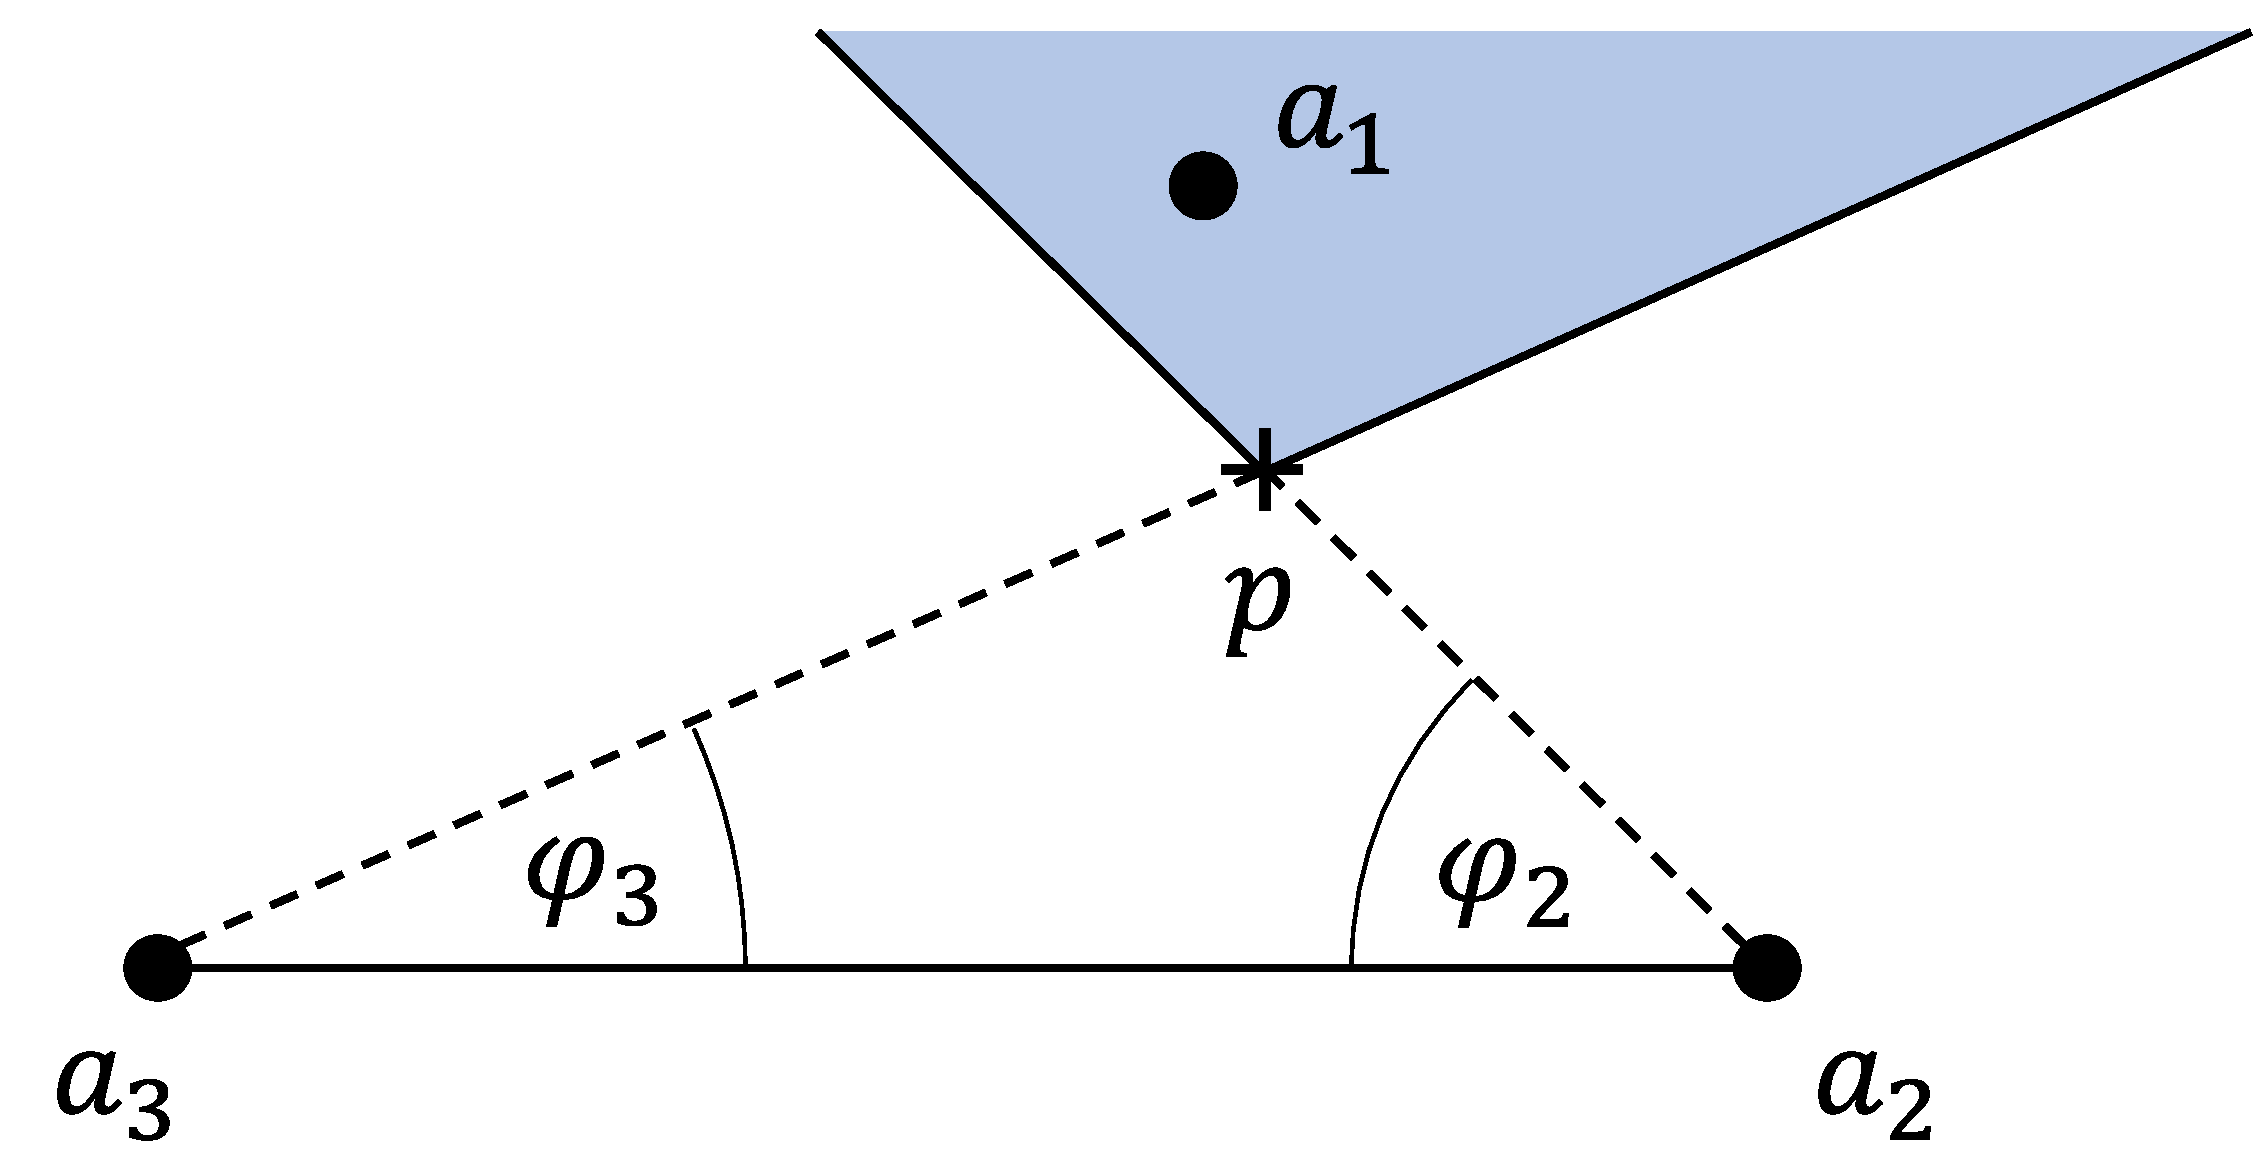
\includegraphics[scale=0.15]{bilder/tri_hilfssatz.pdf}
        \caption{Winkel-Punkteinschluss}
        \label{fig:triangulation_hilfssatz_2}
    \end{figure*}

    Um $p$ nun in einem Dreieck mit $a_2$ und $a_3$ einzuschließen, muss der 
    dreiecksvervollständigende Punkt $a_1$ so liegen, dass gilt:
    $ \{ (a_2,a_3),(a_2,a_1) \} \geq \varphi_2 $ bzw. $ \{ (a_3,a_2),(a_3,a_1) \} \geq \varphi_3 $, 
    denn sonst würde mindestens eine Linie zwischen $p$ und $(a_3,a_2)$ verlaufen, was $p$ 
    ausschließt. Alle Punkte $a_1$, die 
    $ \{ (a_2,a_3),(a_2,a_1) \} \geq \varphi_2 \land \{ (a_3,a_2),(a_3,a_1) \} \geq \varphi_3 $ 
    erfüllen, liegen also per Definition in $f_{a_1}$. $\square$

    \subsubsection{Konstruktion} \label{tri_k}
    Zuerst durchsuche man die Datenpunkte nach dem, an $p$ nächstgelegenen. Dieser ist Teil des 
    Dreiecks minimaler Punktabstandssumme und wir nennen ihn $c$ (\ref{tri_hs1}). Wir teilen die 
    Ebene mit einer Geraden, die durch $c$ und $p$ verläuft. Orthogonal zu dieser legen wir eine 
    weitere Gerade, die durch $p$ geht (in Abb. \ref{fig:konstuktion} rot). 

    \begin{figure*}[!ht]
        \centering	
        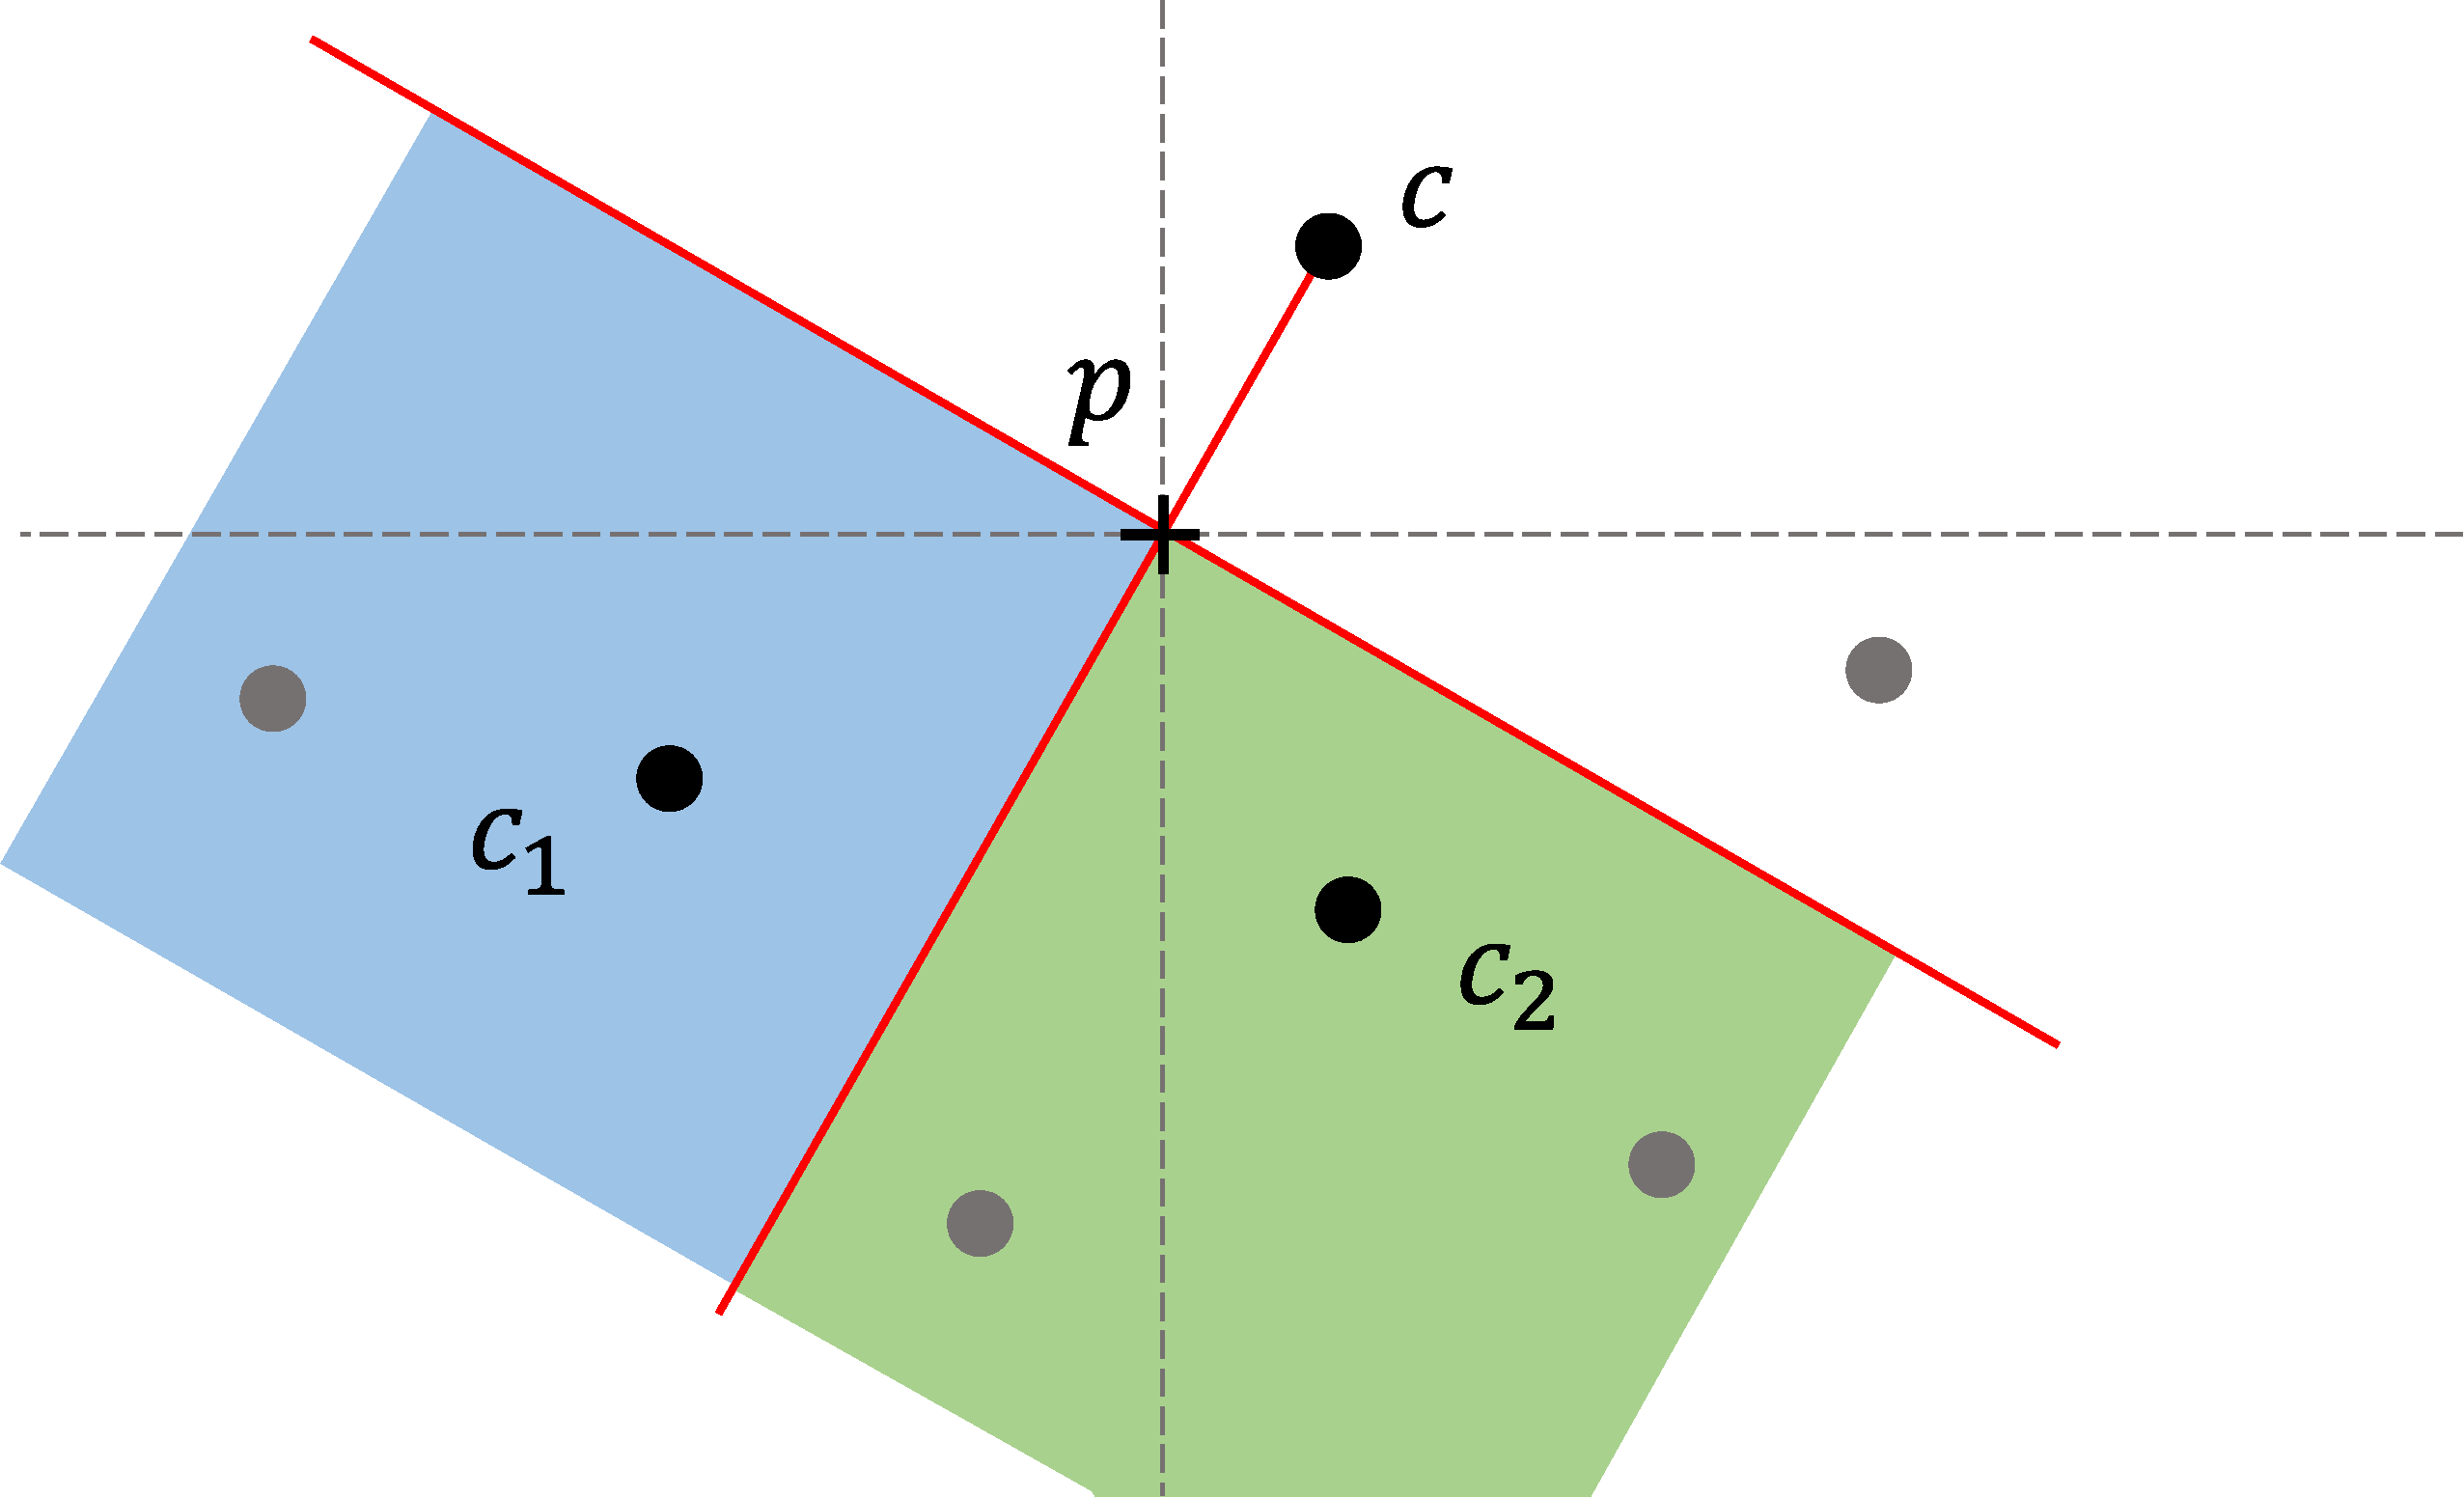
\includegraphics[scale=0.15]{bilder/tri_konstr.pdf}
        \caption{Konstruktion}
        \label{fig:konstuktion}
    \end{figure*}

    Die beiden Quadranten, die nicht an $c$ angrenzen (in Abb. \ref{fig:konstuktion} grün und blau),
    werden verwendet, um Datenpunkte $c_1$ bzw. $c_2$, in jedem der beiden Quadranten einer, zu 
    finden, die mit $c$ ein $p$-umschließendes Dreieck bilden. Dazu nimmt man in beiden Quadranten 
    den nächsten Punkt zu $c$. Die Punkte $c$, $c_1$ und $c_2$ liefern so ein Dreieck mit einer
    einigermaßen kleinen Punktabstandssumme.

    \subsubsection{Laufzeit}
    Der Algorithmus läuft in linearer Laufzeit, da sich das k-kleinste Element einer unsortierten
    Liste in Linearzeit finden lässt. %TODO

    \subsubsection{Selbstkritische Beleuchtung der Konstruktion}
    Die Konstruktion erzeugt schlechte Ergebnisse, falls in mindestens einem der beiden 
    Suchquadranten keine oder sehr weit von $p$ entfernte Datenpunkte liegen, weil die an $c$ 
    angrenzenden Quadranten ignoriert werden, obwohl darin ebenfalls Punkte liegen könnten, die 
    für eine kleinere Punktabstandssumme sorgen würden (siehe Abb. \ref{fig:konstuktion}).
    Ein Lösungsansatz dafür bestünde, indem man beispielsweise zuerst den nächsten Punkt zu $p$ 
    von beiden Quadranten sucht, z.B. $c_1$ und mit diesem dann den möglichen Bereich für $c_2$ 
    absteckt. Dies würde allerdings eine sequentielle Suche nach $c_1$ und $c_2$ verlangen, 
    während unsere Konstruktion Parallelisierung zulässt. \\
    Ein sehr guter Aspekt an der Abstandsminimierung des ersten Punkts $c$ ist, dass, falls $p$ nahe 
    oder auf einem Datenpunkt liegt, die Abweichung von den Messdaten sehr gering ist. \\
    Eine weitere, hervorragende Eigenschaft ist, das sich die Konstruktion in Form eines Algorithmus 
    mit linearer Laufzeit implementieren lässt.
    
    \subsection{Stufe 2 (2HP NN)}
    \begin{itemize}
        \item Generierung einer Grundwahrheit? Warum nicht?
        \item Kommunikation mit dem Modell
        \begin{itemize}
            \item Pipeline / Ablauf einer Anfrage
            \item Optimierungen / Engpässe
        \end{itemize}
    \end{itemize}

    \section{Nutzeroberfläche}

    Unterteilung in Kinderversion und wissenschaftliche Version?
    Farbliche Gestaltung
    
    \subsection{Wissenschaftliche Version}
    \begin{itemize}
        \item Abstriche in der Darstellung
    \end{itemize}

    \subsection{Kinderversion}
    \begin{itemize}
        \item Kinderversion: Nutzernamenvergabe
        \item Einführung und Vereinfachung des Themas für Kinder 
        \item Anreize / Spielifizierung: KI Charakter
        \item Frage: Wie stellt man eine KI dar?
    \end{itemize}
    
    \section{Diskussion}
    \subsection{Nutzeroberfläche}
    \subsection{Backend}
    \subsection{Weiterführende Ideen}

    \section{Fazit}
    
\end{document}